\section{The Ramsey model with endogenous labour supply}
\begin{itemize}
    \item $n = \emptyset$
    \item $g = \emptyset$
    \item $A_0 = \text{Pop}_0 = H = 1$
\end{itemize}

\subsection{Consumption and Leisure}
\begin{equation*}
\begin{aligned}
& \underset{C_t, L_t}{\max}
& & \sum_{t = \tau }^{\infty} (1 + \rho)^{-(t - \tau)} \cdot U(C_t, Z_t) \\
& \text{s.t}
& & K_{t+1} - {K_t} = W_t \cdot L_t + R_t \cdot K_t + \Pi_t - C_t - T_t - \delta K_t \\
\end{aligned}
\end{equation*}

Where $\tau$ represents the period of "today", $Z_t$ is leisure, $\Pi_t$ are are dividends (check in the mail) and $T_t$ is a lump sum tax. All profits in the economy are assumed to be distributed to the households. 

\begin{equation}
Z _ { t } = 1 - L_{ t } \geq 0
\end{equation}
Normalizing the time-endowment to 1. Imagine that $L=0.5$ --- it means that you work half of your time, so $L$ has to be less than 1. 
\begin{equation}
    U(C_t, Z_t) = \frac{C_t^{1 - \theta} - 1}{1 - \theta} + b \frac{(1 - L_t)^{1 - \chi} - 1}{1 - \chi}
\end{equation}
Now the utility function depends on $L$, whereas previously in the Ramsey model we assumed that $L = 1$ and acted as a constant.
\begin{align*}
\theta , \chi > 0 \\
b > 0
\end{align*}

 $\rho > 0$ is the discount rate, and that $\frac{1}{\theta}$
is the the elasticity of inter temporal substitution in Consumption --- $C$ and now we also have $\frac{1}{\chi}$, which is the elasticity of inter temporal substitution in Leisure --- $Z_t$ and the interpretation is the willingness to substitute current consumption or leisure for future consumption or leisure. In \textcite{romer_advanced_2012}
the author assumes that the model is unit-elastic and the elasticities are equal to one. 

\subsubsection*{Current Value Hamiltonian}
Because we are using discrete time instead of continuous time we need to use the current value Hamiltonian 
\begin{multline*}
        H_t = \frac{C_t^{1 - \theta} - 1}{1 - \theta} + b \frac{(1 - L_t)^{1 - \chi} - 1}{1 - \chi} \\ + \lambda_t \bigg[  W_t \cdot L_t + R_t \cdot K_t + \Pi_t - C_t - T_t - \delta K_t \bigg]
\end{multline*}

Obtain the ordinary first order conditions:

\begin{enumerate}[ {(}1{)} ]
    \item 
        $$
            \frac{\partial H_t}{\partial C_t} = \underbrace{C_t^{\theta} - \lambda_t}_{MU C_t} = 0
        $$
        Where $\text{MUC}_t$ is the marginal utility of consumption
            \item 
        $$
            \frac{\partial H_t}{\partial L_t} = \underbrace{-b (1- L_t)^{ - \chi} + \lambda_t W_t}_{MU Z_t} = 0
        $$
        Where $MU Z_t$ is the marginal utility of leizure 
                    \item 
        $$
            \frac{\partial H}{\partial K_t} = \lambda_{t+1} (R_{t+1} - \delta) = - (\lambda_t - \lambda_{t-1}) + \rho \lambda_{t - 1} 
        $$
                            \item 
        $$
            \lim_{t\to\infty} \bigg[ (1 + \rho )^{\tau} \cdot \lambda_t \cdot K_{t+1} \bigg] = 0
        $$
        The transversality condition
\end{enumerate}

By solving (1) for $\lambda_t$, and write $\lambda_{t+1}$ we get:
$$
\lambda_t = C_t^{-\theta} \implies \lambda_{t+1}=C_{t+1}^{-\theta}
$$

Initially (3) is written in a way that allows to chose the capital stock, however, that is not possible as it is a predetermined variable and the equation is therefore not valid for the current time period, only the future. We therefore need to write it in terms of period $t+1$, thus:
        $$
        \lambda_{t+1} (R_{t+1} - \delta) = - (\lambda_{t+1} - \lambda_{t-1}) + \rho \lambda_{t}
        $$
        
By rearranging and substituting the expression for $\lambda_{t+1}$ we got from (1) we obtain:

$$
C_{t+1}^{-\theta} (1 + R_{t+1}) = (1 + \rho)C_{t+1}^{-\theta}
$$


\begin{equation*}
    \frac {  C_{t+1}  } { C_t }  = \left( \frac { 1 + \rho } { 1 + R _ { t + 1 } } \right) ^ { 1 - \theta }
\end{equation*}

Which is the Consumption Euler Equation like we saw in the OLG-model. 

By using (2) we can substitute for $\lambda_t$:
$$
-b (1- L_t)^{1 - \chi} + C_{t}^{-\theta} W_t = 0 \implies b(1 - L_t)^{- \chi } = C_t^{-\theta} W_{t}
$$
We can now solve this for $L_t$ to get:

\begin{equation}\label{frisch_labour_supply}
    L_t = 1 - \left( \frac{C_t^{-\theta}W_t}{b} \right) ^{-\frac{1}{\chi}}
\end{equation}

Which is called the Frisch labour Supply function, which is not really a labour supply function

MRS of $C_t$ and $Z_t$

$$
\frac{\partial L_t}{\partial W_t} = \frac{1}{\chi} \cdot \frac{C_t^{- \theta}}{b} \left( \frac{C_t^{- \theta} W_t}{b} \right) ^ {- \frac{1}{\chi} -1 } > 0
$$

Where $\tfrac{\partial L_t}{\partial W_t}$ is the Substitution Effect (SE) and $\tfrac{\partial^2 L_t}{\partial^2 W_t}$ is the Wealth Effect (WE)

$$
\frac{\partial L_t}{\partial L_t} = - \frac{\theta}{\chi} \cdot \frac{C_t^{- \theta - 1}}{b} \left( \frac{C_t^{- \theta} W_t}{b} \right) ^ {- \frac{1}{\chi} -1 } < 0
$$

There is a S.S where
$$
r^* = \rho 
$$

or $C^* = 0$

$$
R^* - \delta = \rho \implies R^* = \rho - \delta
$$
The rental price of capital is equal to the discount rate plus the depreciation rate

\subsubsection{The Firms Problem}

$$
R_t = MPK_t = \frac{\partial Y_t}{\partial K_t} = \alpha \left( \frac{A_t L_t}{K_t} \right)^{1-\alpha}
$$

$$
W_t = MPL_t = \frac{\partial Y_t}{\partial L_t} = (1 - \alpha ) A_t^{1-\alpha} \left( \frac{K_t}{L_t} \right)^{\alpha} 
$$

\subsubsection{Equilibrium in the labour market}

By substituting the expression for $W_t$ into the Frisch Labour Supply Function --- \ref{frisch_labour_supply} we can obtain an equilibrium equation:

\begin{equation*}
        L_t = 1 - \left[ \frac{(1 - \alpha ) A_t^{1-\alpha} \left( \frac{K_t}{L_t} \right)^{\alpha}}{b} \right] ^{-\frac{1}{\chi}}  \cdot C_t^{- \frac{\theta}{\chi}}
\end{equation*}

Unless $\theta$ and $\chi$ are equal to 1 there is no closed-form solution for $L_t$ for this equation, but we can write it as an implicit function as:

$$
L_t = \mathcal{L} (K_t, C_t, A_t)
$$

This is the employment equilibrium as a function of $K_t, C_t, A_t$

The partial derivatives gives us useful information regarding changes in the variables

$$
\frac{\partial \mathcal{L}}{\partial K} = \frac{\alpha (1- L^*)}{\chi K^* \cdot \Phi^*} > 0
$$

An increase in the capital stock gives rise to an increase in employment.

$$
\frac{\partial \mathcal{L}}{\partial C} = \frac{- \theta ( 1 - L^*)}{\chi C^* \cdot \Phi ^* } < 0
$$

Increased consumption leads to a decrease in employment.

$$
\frac{\partial \mathcal{L}}{\partial A} = \frac{(1 - \alpha) (1 - L^*)}{\chi A^* \phi^*} > 0
$$

$$
\phi^* = 1 + \frac{1-L^*}{L*} \cdot \frac{\alpha}{\chi} > 1
$$

$$
R_t = \text{MPK}_t = \text{MPK}(K_t, L_t, A_t) = \text{MPK} \left[ K_t, \mathcal{L}(K_t, L_t, A_t), A_t \right] = \mathcal{R} (K_t, C_t, A_t)
$$

Derivatives of $\mathcal{R}$

$$
\frac{\partial \mathcal{R}}{\partial K} = - \frac{L^*}{K^{* 2} \Phi^*} < 0
$$

$$
\frac{\partial \mathcal{R}}{\partial C} =  \frac{\partial \text{MPK}}{\partial L} \cdot \frac{\partial L}{\partial C} < 0
$$

$$
\frac{\partial \mathcal{R}}{\partial A} =  \frac{\partial \text{MPK}}{\partial A} \cdot L^* + A^\alpha \cdot \frac{\partial \text{MPK}}{\partial L} \cdot \frac{\partial \mathcal{L}}{\partial A} > 0
$$




\begin{figure}[ht]
\centering
\begin{subfigure}{.5\textwidth}
  \centering
  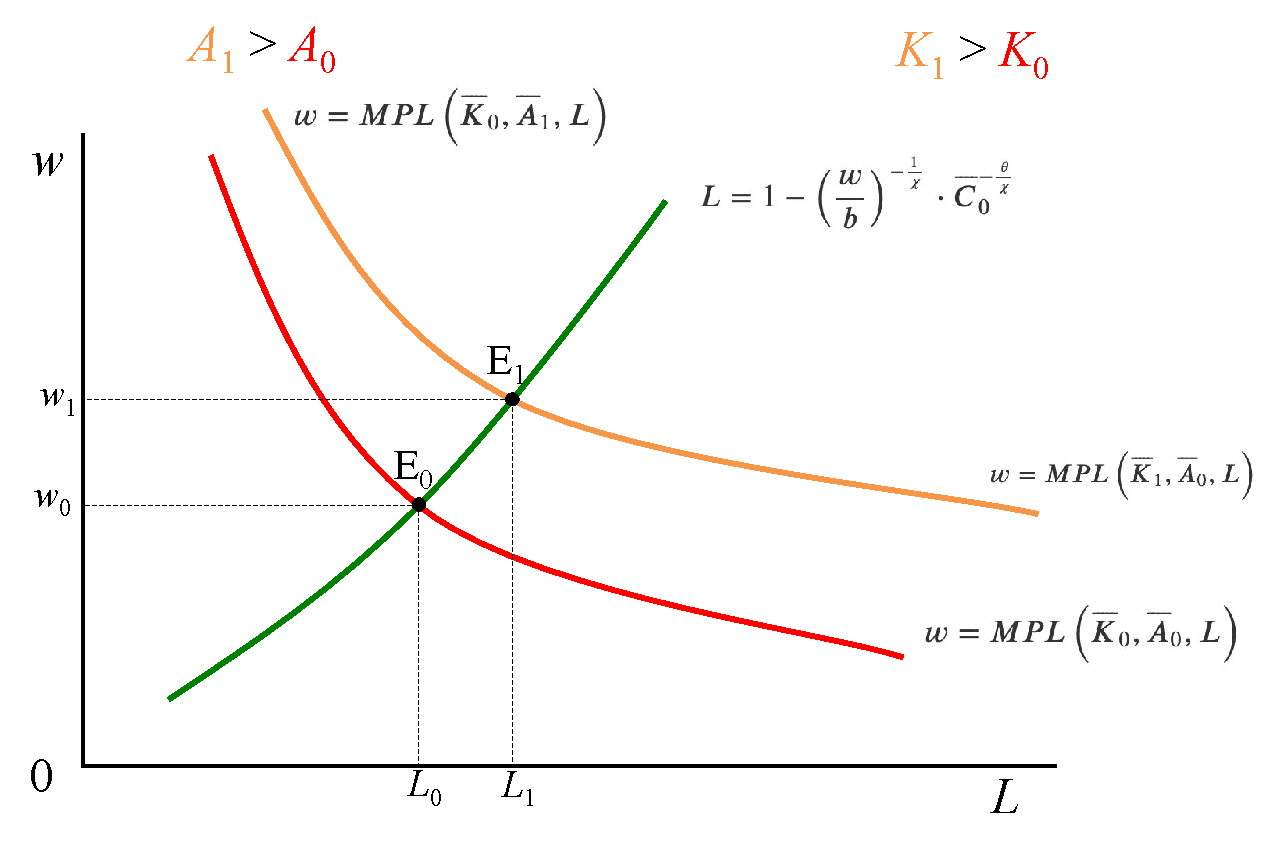
\includegraphics[width=1\linewidth]{3_0_Real_Business_Cycles/e_q_L_1.pdf}
  \caption{Case 1}
  \label{fig:sub1}
\end{subfigure}%
\begin{subfigure}{.5\textwidth}
  \centering
  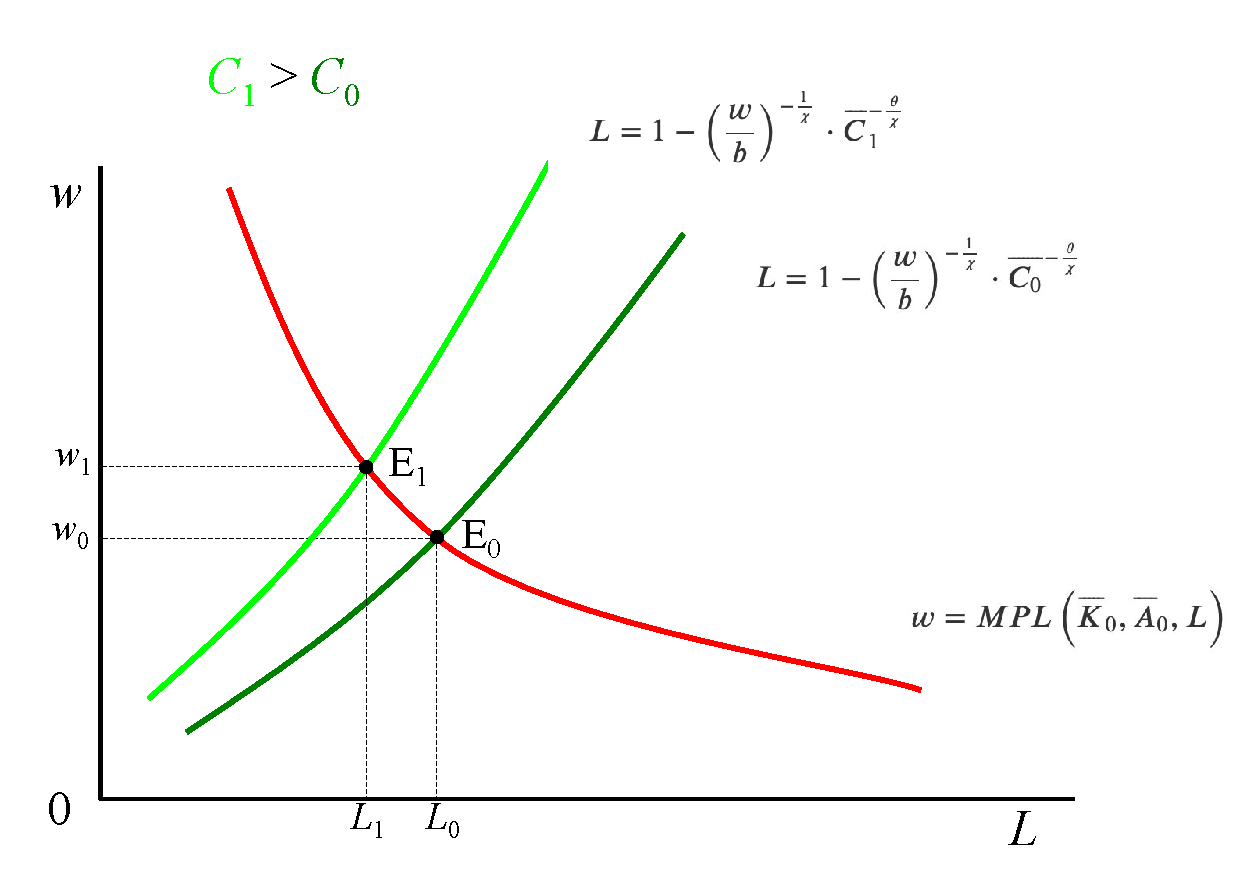
\includegraphics[width=1\linewidth]{3_0_Real_Business_Cycles/e_q_L_2.pdf}
  \caption{Case 2}
  \label{fig:sub2}
\end{subfigure}
\caption{Equilibrium in the Labour Market}
\label{fig:test}
\end{figure}

A.t S.s

\begin{equation*}
   R ^ { * } = \rho + \delta \implies  R \left( K ^ { * } , C^ { * } , A ^ { * } \right) = \rho + \delta \implies 
   \alpha \left[  \frac{A^* \cdot \mathcal{L}(K^*, C^*, A^*)}{K^*}  \right]^{1 - \alpha} = \rho + \delta
\end{equation*}

\paragraph{Steady Steady Consumption:}

$$
C^* = \mathcal{C} \left( K^*, A^*, \rho + \delta \right)
$$

$$
\frac{\partial \mathcal{C}}{\partial K} = - \frac{\frac{\partial \mathcal{R}}{\partial K}}{\frac{\mathcal{R}}{\partial C}} < 0
$$

The larger the capital stock, the larger the consumption at the steady state. 


$$
\frac{\partial \mathcal{C}}{\partial A} = - \frac{\frac{\partial \mathcal{R}}{\partial A}}{\frac{\mathcal{R}}{\partial C}} > 0
$$

Productivity is good for consumption at the steady state. 



$$
\frac{\partial \mathcal{R}}{(\rho + \delta)} = \frac{\frac{1}{\partial \mathcal{R}}}{\partial C} < 0
$$

The larger the deprecation rate, the lower the consumption at the steady state. 

There is a negative relationship

\subsection{Capital Accumulation}

$$
\Delta K_{t + 1} = WtLt + R_t K_t + \Pi_t - C_t - T_t - \delta K_t
$$

We have $\Pi = 0$ and $\Pi_t = G_t$


Output is given by: 
$$
Y = W_t L_t + R_t K_t
$$

$$
K_t^{\alpha} \cdot \left( A_t L_t \right)^{1 - \alpha} - C_t - \delta K_t - G_t
$$

Recall that $L_t$ is the labour supply function $\mathcal{L}(K_t, C_t, A_t)$

Thus we can replace to get:
$$
K_t^{\alpha} \cdot \left( A_t \cdot \mathcal{L}(K_t, C_t, A_t) \right)^{1 - \alpha} - C_t - \delta K_t - G_t
$$
We have the following derivatives of $\mathcal{L}$:

\begin{align*}
    \frac{\partial \mathcal{L} }{\partial K_t} > 0 && \frac{\partial \mathcal{L}}{\partial C_t} < 0 && \frac{\partial \mathcal{L} }{\partial A_t} > 0
\end{align*}

Long run equilibrium + dynamic

Permanent shocks:
\begin{enumerate}[a)]
    \item Productivity shocks
    \item Fiscal Policy shocks
\end{enumerate}
